\documentclass{beamer}
\mode<presentation>
\usetheme{CambridgeUS}
\usepackage[russian]{babel}
\usepackage[utf8]{inputenc}
\usepackage[T2A]{fontenc}
\usepackage{sansmathaccent}

\usepackage{verbatim}
\usepackage{alltt}

\pdfmapfile{+sansmathaccent.map}
\title[Массивы]{Массивы}
\author{Наумов Д.А., доц. каф. ИТГД}
\date[14.02.2020] {Алгоритмические языки и программирование, 2020}

\begin{document}

%ТИТУЛЬНЫЙ СЛАЙД
\begin{frame}
  \titlepage
\end{frame}
  
%СОДЕРЖАНИЕ ЛЕКЦИИ
\begin{frame}
  \frametitle{Содержание лекции}
  \tableofcontents  
\end{frame}
  
\section{Массив}
\subsection{Определение, описание, модель}
\begin{frame}[fragile]
\textbf{Массив} ~-- упорядоченный набор однотипных элементов (компонентов массива), доступ к которым осуществляется при помощи индекса.
Основные характеристики массива:
\begin{itemize}
\item размерность (одномерный, двухмерный и т.д.);
\item тип индексов;
\item тип элементов;
\end{itemize}
\begin{alltt}
(* Описание типа одномерного массива *)
1  type ИмяТипа = array[ТипыИндексов] of ТипЭлемента;
2  var ИмяПеременной1: ИмяТипа;
(* Описание переменной-массива *)
3  var ИмяПеременной2: array[ТипыИндексов] of ТипЭлемента;
\end{alltt}
\end{frame}

\begin{frame}[fragile]
Доступ к элементам массива осуществляется при помощи индексов. Тип индексов может быть любым порядковым типом:
\begin{itemize}
\item целым (byte, shortint, integer, word);
\item символьным (char);
\item логическим (boolean);
\item перечисляемым;
\item отрезковым.
\end{itemize}
\begin{alltt}
1 type
2    digit = array[0..9] of char; (*одномерный массив*)
(* двухмерный массив *)
3    matrix = array[byte, 'A'..'D'] of real;  
4 var
5    A, B : digit;
6    M1, M2 : matrix; 
(* трехмерный массив *)
7    Cube : array[1..5, 'A'..'H', boolean] of char; 
\end{alltt}
\end{frame}

\begin{frame}
Массивы могут использовать для представления списка или вектора (одномерный массив), матрицы (двумерный массив), и т.д. 
\begin{figure}[h]
\centering
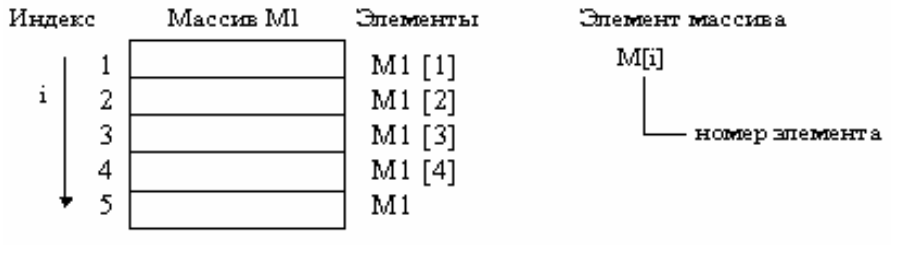
\includegraphics[scale=0.5]{images/one_index.png}
\caption{Одномерный массив}
\label{pic-one-index}
\end{figure}
\end{frame}

\begin{frame}
Массивы могут использовать для представления списка или вектора (одномерный массив), матрицы (двумерный массив), и т.д. 
\begin{figure}[h]
\centering
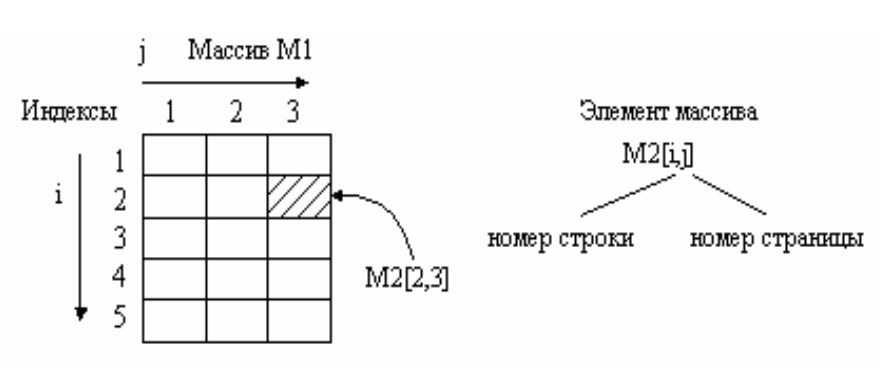
\includegraphics[scale=0.5]{images/two_index.png}
\caption{Двумерный массив}
\label{pic-two-index}
\end{figure}
\end{frame}

\subsection{Операция индексации}
\begin{frame}[fragile]
Доступ к отдельному элементу массива осуществляется при помощи операции индексации: указанием идентификатора массива, за которым в квадратных скобках указаны выражения, тип значения и количество которых соответствуют типам индексов.
\begin{alltt}
1 type Fam = (Ivanov, Petrov, Sidorov);
2   TMark = 2..5; 
3 var 
4   MarksAvg: array[Fam] of real;
5   Group741, Group748: array[1..30] of TMark;
6   i, j, k: integer;
\end{alltt}
К компонентам массива применимы операции и функции, допустимые для переменной базового типа. 
\begin{alltt}
1 i := 15; j := 20; k := 10;
2 MarksAvg[ Ivanov ] := 4.75;
3 Group741[i] := Group748[j - k];
(* допустимо при совпаднии типов индексов и элементов *)
4 Group848 := Group841; 
\end{alltt}
\end{frame}

\subsection{Типовые операции с массивом}
\begin{frame}
Ввод элементов одномерного массива при помощи цикла с параметром.
\begin{figure}[h]
\centering
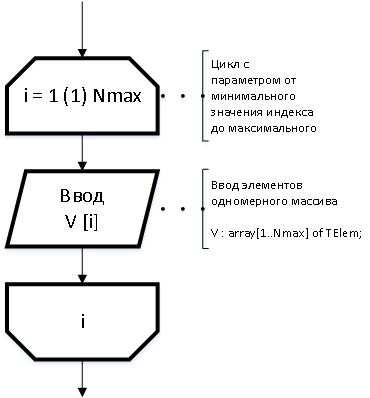
\includegraphics[scale=0.5]{images/array_input.png}
\caption{Ввод элементов одномерного массива}
\label{pic-input-one-index}
\end{figure}
\end{frame}

\begin{frame}
Ввод элементов одномерного массива при помощи цикла с параметром.
\begin{figure}[h]
\centering
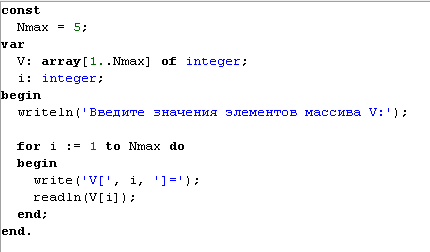
\includegraphics[scale=1.0]{images/array_input_code_one.png}
\caption{Ввод элементов одномерного массива}
\label{pic-input-one-index-code}
\end{figure}
\end{frame}

\begin{frame}
Ввод элементов двумерного массива при помощи вложенный циклов.
\begin{figure}[h]
\centering
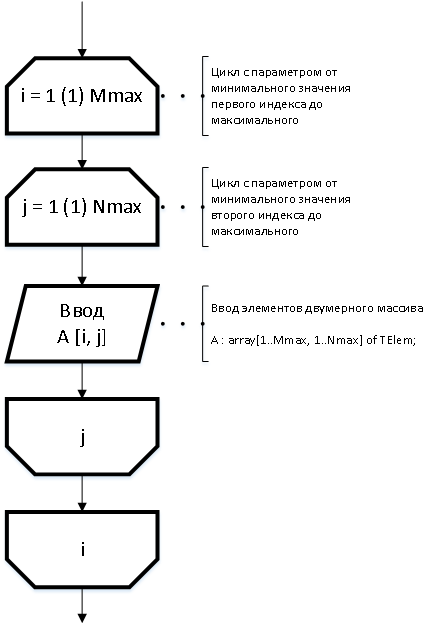
\includegraphics[scale=0.45]{images/array_input_two.png}
\caption{Ввод элементов двумерного массива}
\label{pic-input-two-index}
\end{figure}
\end{frame}

\begin{frame}
Ввод элементов двумерного массива при помощи вложенных циклов.
\begin{figure}[h]
\centering
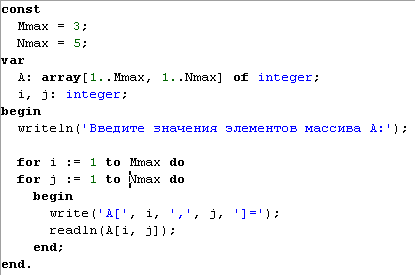
\includegraphics[scale=1.0]{images/array_input_code_two.png}
\caption{Ввод элементов двумерного массива}
\label{pic-input-two-index-code}
\end{figure}
\end{frame}

\begin{frame}
Вывод элементов одномерного массива.
\begin{figure}[h]
\centering
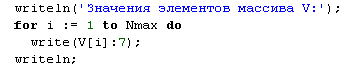
\includegraphics[scale=1.0]{images/array_output_code_one.png}
\caption{Вывод элементов одномерного массива}
\label{pic-output-code-one}
\end{figure}

Вывод элементов двумерного массива.
\begin{figure}[h]
\centering
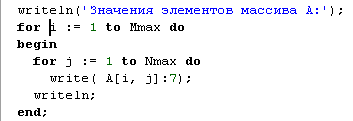
\includegraphics[scale=1.0]{images/array_output_code.png}
\caption{Вывод элементов двумерного массива}
\label{pic-output-code-two}
\end{figure}
\end{frame}

\begin{frame}
В одномерном массиве М, состоящем из N целых чисел, найти элементы, значения которых равны заданному числу K.
\begin{figure}[h]
\centering
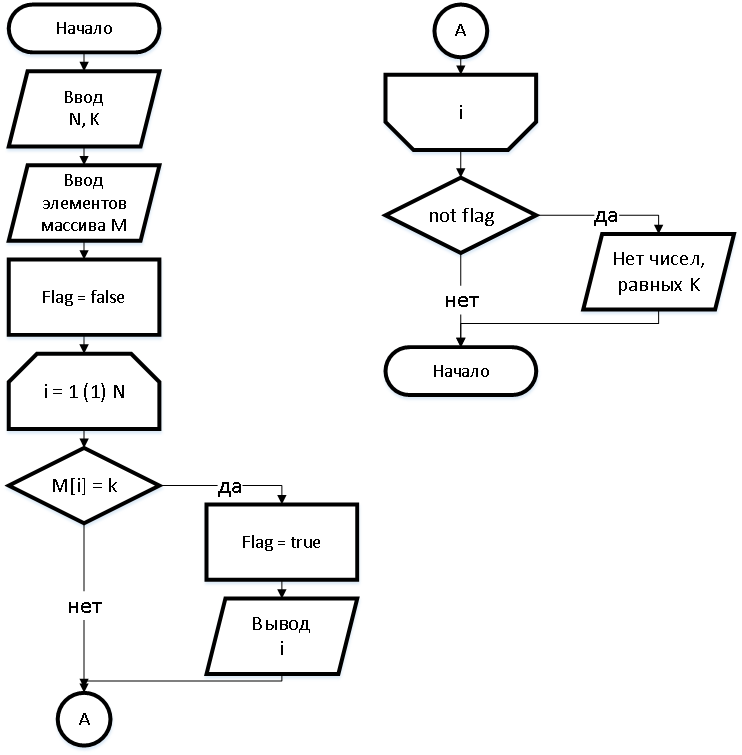
\includegraphics[scale=0.35]{images/array_search.png}
\caption{Поиск элементов в одномерном массиве}
\label{pic-search}
\end{figure}
\end{frame}

\begin{frame}
В одномерном массиве М, состоящем из N целых чисел, найти элементы, значения которых равны заданному числу K.
\begin{figure}[h]
\centering
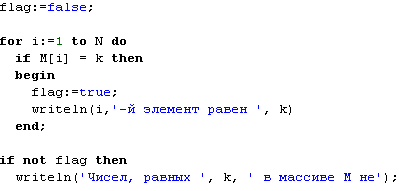
\includegraphics[scale=1.0]{images/array_search_code.png}
\label{pic-search-code}
\end{figure}
\end{frame}

\begin{frame}
В одномерном массиве М, состоящем из N целых чисел, найти минимальное значение элемента.
\begin{figure}[h]
\centering
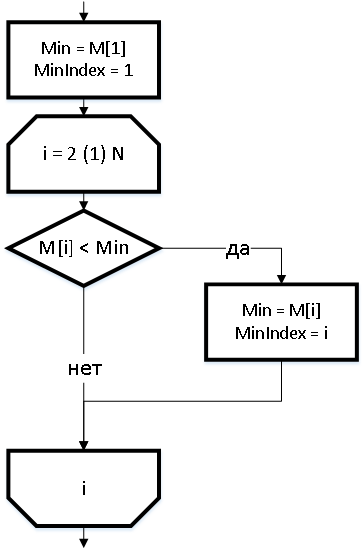
\includegraphics[scale=0.35]{images/array_min.png}
\caption{Поиск минимального элемента в одномерном массиве}
\label{pic-search}
\end{figure}
\end{frame}

\begin{frame}
В одномерном массиве М, состоящем из N целых чисел, найти минимальное значение элемента.
\begin{figure}[h]
\centering
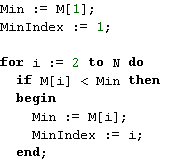
\includegraphics[scale=1.0]{images/array_min_code.png}
\label{pic-search-code}
\end{figure}
\end{frame}

\begin{frame}
Для обмена значениями двух элементов массива необходимо использовать вспомогательную переменную для временного хранения одного из элементов.
\begin{figure}[h]
\centering
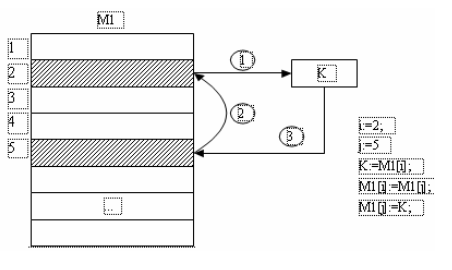
\includegraphics[scale=0.8]{images/array_swap.png}
\label{pic-search-swap}
\end{figure}
\end{frame}

\begin{frame}
Типовой задачей является сортировка элементов массива.
\begin{figure}[h]
\centering
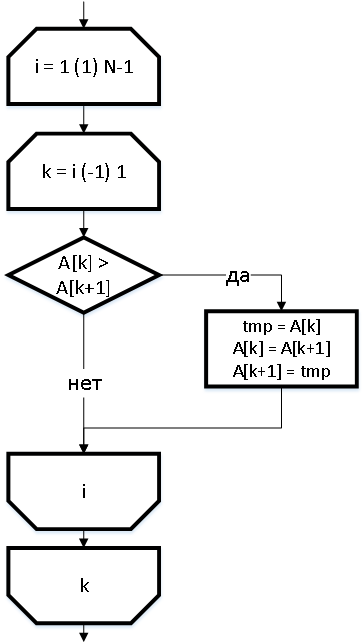
\includegraphics[scale=0.4]{images/array_sort.png}
\label{pic-sort}
\end{figure}
\end{frame}

\begin{frame}
Фрагмент кода для сортировки методом "пузырька".
\begin{figure}[h]
\centering
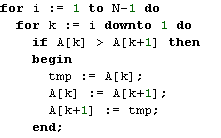
\includegraphics[scale=1.0]{images/array_sort_code.png}
\label{pic-sort}
\end{figure}
\end{frame}

\begin{frame}[fragile]
Объявление констант типа массив позволяет задать значение компонент неизменяемого массива.
\begin{alltt}
1  Type Status = (Active, Passive, Waiting); 
2    StatusMap = Array [Status] Of String[7];
3  Const StatStr : StatusMap = ('Active', 'Passive', 'Waiting');
\end{alltt}
Упакованные константы со строковым типом (символьные массивы) могут быть определены и как одиночные символы, и как строки.
\begin{alltt}
4  Const Digits1 : array [0..9] Of Char 
         = ('0', '1', '2', '3', '4', '5','6', '7', '8', '9'); 
5  Const Digits2 : array [0..9] Of Char = '0123456789';
\end{alltt}
Константы - многомерные массивы определяются заключением констант каждой размерности в отдельные наборы круглых скобок, разделенные запятыми.
\begin{alltt}
6  Type Cube = array[0..1, 0..1, 0..1] Of Integer;
7  Const Array_Maze : cube = 
     (((0, 1), (2, 3)), ((4, 5), (6, 7)));
\end{alltt}
\end{frame}

\begin{frame}[fragile]{Упражнения}
В следующих задачах переменные x, y, z описаны как 
\begin{alltt}
var x, y, z: array[1..n] of integer;
\end{alltt}
\begin{enumerate}
\item заполнить массив х нулями;
\item подсчитать количество нулей в массиве;
\item присвоить значение элементов массива x массиву y;
\item найти максимум в массиве x;
\item дан массив x, причем x[1]<=x[2]<=...<=x[n]. Найти количество различных элементов этого массива
\item найти количество различных элементов в массиве х
\item переставить элементы в массиве х в обратном порядке
\item дан массив x[m+n], рассматриваемый как соединение отрезков x[1]...x[m] и x[m+1]...x[m+n]. не используя дополнительных массивов, переставить начало и конец массива x
\item даны два возрастающих массива. найти количество их общих элементов
\end{enumerate}
\end{frame}   
   
\section*{Литература}
\begin{frame}   
\begin{enumerate}
\item Алгоритмические языки и основы программирования: Учебное пособие / В.Д.Былкин, Ю.В Блинков, Т.А. Глебова, В.В. Пикулин / Под общ ред. проф. А.Н.Кошева. - Пенза: ПГУAC, 2004. - 280 с. ISBN 5-9282-022J-0
\end{enumerate}
\end{frame}   

\end{document}
